\documentclass[14pt, a4paper]{report}
\usepackage{mathtext}
\usepackage[T2A]{fontenc}
\usepackage[utf8]{inputenc}
\usepackage[russian]{babel}
\usepackage{multirow}
\usepackage{slashbox}
\usepackage{makecell}
\usepackage{graphicx}
\usepackage{physics}
\usepackage{amstext}
\usepackage{caption}
\usepackage{subcaption}
\usepackage{cmap}
\usepackage{float}

\renewcommand{\thesection}{\arabic{section}.}
\renewcommand{\thesubsection}{\arabic{section}.\arabic{subsection}.}

\title{\textbf{Отчет о выполнении лабораторной работы 4.5.1 "Гелий-неоновый лазер"}}
\author{Алпатова Александра, Калашников Михаил, Б03-205}
\date{}

\begin{document}
\maketitle

\textbf{Цель работы:}
изучение основных принципов работы гелий-неонового лазера, свойств лазерного излучения и измерение усиления лазерной трубки.
\newline

\textbf{В работе используются:}
\begin{itemize}
\item объект исследования -- активный элементот гелий-неонового лазера ЛГ-75 с блоком питания;
\item дополнительный He–Ne-лазер для юстировки и измерений;
\item модулятор излучения (обтюратор);
\item фотодиоды;
\item зеркала;
\item поляроид;
\item компьютер со звуковой картой.
\end{itemize}

\section{Теоретические сведения}

\section{Экспериментальная установка}

\section{Проведение эксперимента и обработка данных}

\begin{enumerate}

\setcounter{enumi}{0}

\item Включим питание юстировочного лазера.

\item Проведем юстировку оптической схемы установки. Получим на экране равномерно освещенный пучок света.

\item Измерим усиление трубки. Повернем глухое зеркало так, чтобы проходящий через трубку пучок попадал на второй фотодиод. Включим мотор модулятора. Проведем измерение отношения сигналов с первого и второго фотодиодов. Полученное значение близко к 1.5.

\item Добьемся лазерной генерации, повернув глухое зеркало параллельно полупрозрачному зеркалу.

\item Исследуем состояние поляризации лазерного луча на исследуемой трубке с помощью поляризационной пластинки. Для этого будем вращать пластинку и отмечать показания фотодиода. Полученную зависимость представим на графике. Сверху наложим функцию $y=a\sin{x-b}^2$.

\begin{figure}[H]
\centering
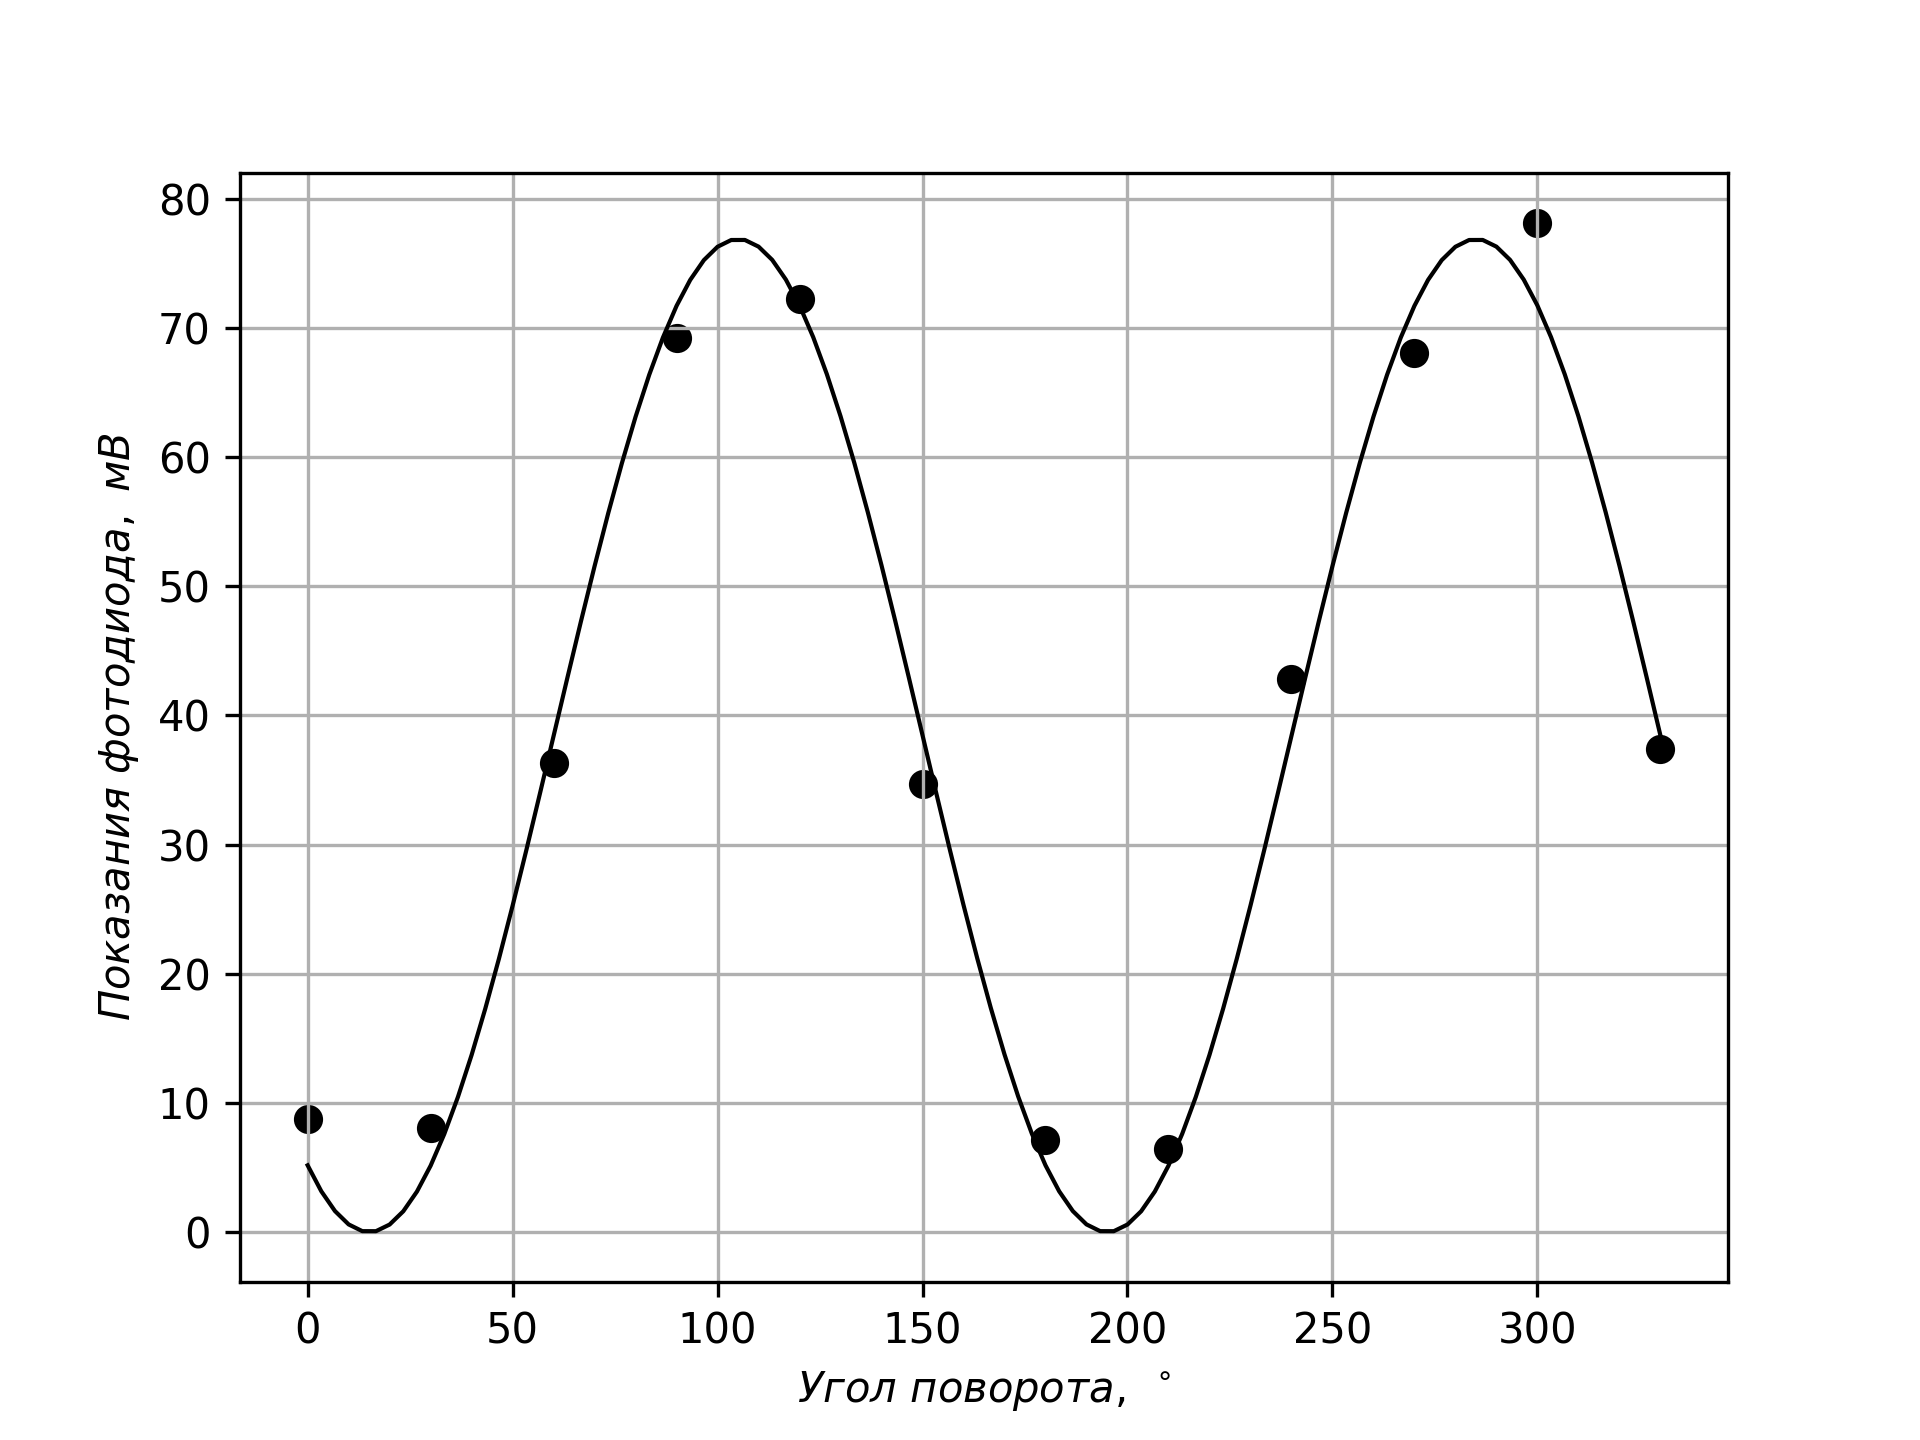
\includegraphics[scale=0.6]{images/451_1.png}
\caption{Показания фотодиода при вращении поляризационной пластинки}
\end{figure}


\end{enumerate}

\section{Вывод}





\end{document}